
% !TEX root = NotesDeCours.tex

%\setcounter{section}{0}

%\part{Introduction -- Analyse dimensionnelle}
\nohandout{\section{Introduction -- Analyse dimensionnelle}}

% ================================================================================================ 
% Page de titre :
% ================================================================================================

\begin{frame}

  \color{bleu}

  \begin{flushleft}
    
    \Large
   	\bf
    
    Mécanique des fluides 

  \end{flushleft}
  
  \ligne{3} % remplace: \noindent \thickline{0.5mm}{150}

  \begin{flushright}

    \rm

    \textrm{David} \textsc{Fabre}
    
    \vspace{3mm}
    
    IMFT / UPS
    
    Département de Mécanique
    
  %  brancher@imft.fr

  \end{flushright}

%\begin{picture}(110, 22)(-9, 5)
 % \put( 0, 25){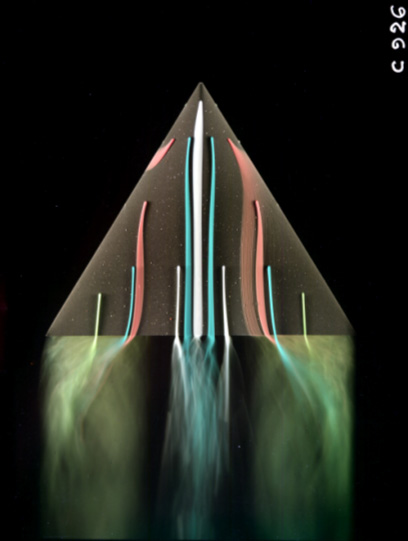
\includegraphics[width=30mm]{./Figures/Werle_aileDelta.jpeg}}
 % \put( 6,  0){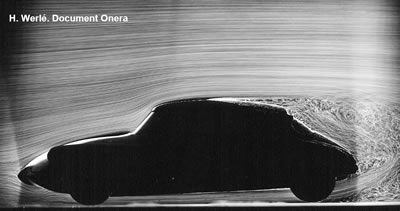
\includegraphics[width=40mm]{./Figures/Werle_Voiture.jpeg}}
  %\put( 0, 23){\color{gris} \small \rm Lignes d'émission dans le sillage d'une maquette d'avion de %type "aile delta" } 
 % \put( 0, 20){\color{gris} \small \rm }
 % \put( 0,  -3){\color{gris} \small \rm Ecoulement dans le sillage d'une maquette d'automobile}
 % \put( 0, -6){\color{gris} \small \rm }
%\end{picture}

\begin{tabular}{cc}
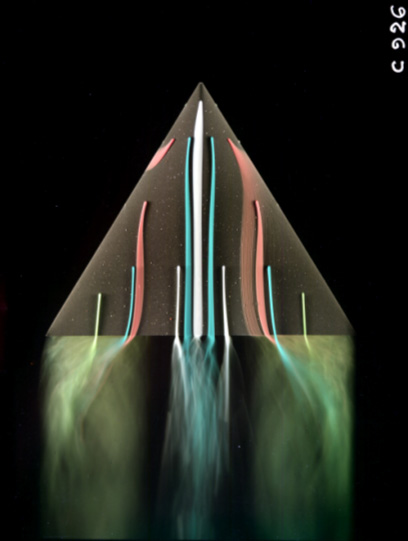
\includegraphics[width=20mm]{./Figures/Werle_aileDelta.jpeg}
&
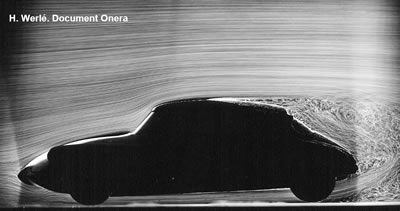
\includegraphics[width=40mm]{./Figures/Werle_Voiture.jpeg}
\\
\small Lignes d'émission dans le sillage  
&
\small Ecoulement dans le sillage 
\\
\small d'une maquette d'avion de type "aile delta"
&
\small d'une maquette d'automobile
\end{tabular}

\medskip
{\small \color{gray}
Images : expériences en tunnel hydrodynamique, H. Werlé (ONERA)
}

  \vspace{12mm}
  
  \begin{flushright}
    
    \Large
   	\bf
    
    1. Introduction -- Analyse dimensionnelle

  \end{flushright}

\end{frame}

%%%%%%%%%%%%%%%%%%%%%%%%%%%%%%%%%%%%%%%%%%%%%%%%%%%%%%%%%%%%%%%%%%%%%%%%%%%%%%%%%%%%%%%%%%
% Sommaire :
%%%%%%%%%%%%%%%%%%%%%%%%%%%%%%%%%%%%%%%%%%%%%%%%%%%%%%%%%%%%%%%%%%%%%%%%%%%%%%%%%%%%%%%%%%


\begin{frame}{Sommaire}

\small
  
\hspace*{2mm}
\begin{tabular}{cc}
		%&
  		\begin{minipage}{62mm}
  			\tableofcontents[firstsection=0]
      \vspace{15mm}
  		\end{minipage}
  		&   
  		\begin{minipage}{60cm}
		  \vspace*{-5mm}  
  			%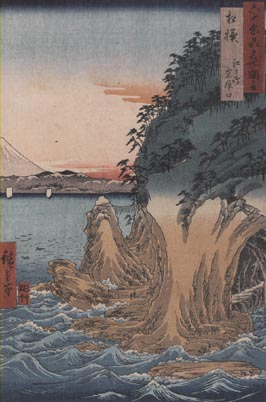
\includegraphics[width=40mm]{vagues.jpg} 
  		\end{minipage}
  	\end{tabular}

\vspace{0mm}

\end{frame}






%==================================================================================================
\subsection{Introduction : Qu'est-ce qu'un fluide ?}
%==================================================================================================

%--------------------------------------------------------------------------------------------------
\begin{frame}{Le millieu fluide : définition \ldots}
%--------------------------------------------------------------------------------------------------

\small

\textbf{Point de vue du thermodynamicien :} \bigskip

Pour un corps pur on appelle phases fluides les deux états fondamentaux suivants : 

\pause

\medskip

\begin{itemize}[<+-| alert@+>]
\item
	gaz (vapeur) : \textrm{O$_2$}, \textrm{CO$_2$}, \textrm{He}, etc.
\item
	liquide : \textrm{H$_2$O}, métaux liquides (\textrm{Hg} à température ambiante, 
	\textrm{Zn} pour $T>450^o C$, \\
	\textrm{Fe} liquide comme dans le noyau liquide de la Terre, ... )
	%dont les mouvements par effet dynamo %sont à l'origine du champ magnétique terrestre)

\item Plus deux états qui ne sont pas des phases bien définies :
	
$\rightarrow$ 
Fluides supercritiques. 
	
$\rightarrow$
	Plasmas (gaz composé d'ions et d'électrons) : 
	haute atmosphère, étoiles (estimation : 99\% de la matière de l'Univers)

\end{itemize}


\pause


\textbf{Point de vue du mécanicien :} \bigskip

Fluide = tout matériau susceptible de s'écouler ; cad de se déformer continument sous l'effet de forces extérieures.


%\medskip

%\textbf{Point de vue du chimiste :} \bigskip

\textbf{
De ce point de vue un fluide être un mélange de corps purs (fluides ou non) :}

\pause

\medskip

\begin{itemize}[<+-| alert@+>]
\item
	mélange de gaz (ex. air : mélange oxygène et azote principalement)

\item mélange de liquides miscibles	
	( pastis = eau+alcool,...) ou solutions (eau de mer, perrier...)

\item Mélanges de liquides non miscibles (ex. eau et huile, vinaigrette)

\item Suspensions (lait, etc...)

\item Collection de corps célestes (anneaux de saturne, galaxies,...)
	
\end{itemize}

%\vspace{15mm}

\end{frame}



\subsection{Modélisation d'un fluide}

\subsubsection{Description microscopique et description MMC}


%--------------------------------------------------------------------------------------------------
\begin{frame}{Modélisation d'un fluide :}
%--------------------------------------------------------------------------------------------------

\small

Deux types de modélisation possibles:
\pause
\begin{enumerate}
\item Modélisation à l'échelle microscopique (échelle $\ell$ caractéristique des interactions intermoléculaires) :

On s'intéresse à la {\em vitesse individuelle} $\vec v_i$ de chacune des particules constituant le fluide 
$(i = 1...N)$


$=>$ On peut alors écrire un {\em système d'équations différentielles (discret)}, de grande dimension, de la forme $d \vec{v}_i / dt = ....$ 
 

\pause
\item Modélisation à l'échelle (échelle $L$) : 

On s'intéresse à la  {\em vitesse moyenne} $\vec{u}(\vec x)$ 
des particules se trouvant au voisinage d'un point de coordonnées $\vec x$ :  {\em vitesse au sens de la MMC}

$=>$ On cherche alors à écrire un {\em système d'équations aux dérivées partielles (continu)} 

de la forme $d \vec u / dt = ....$ 

\end{enumerate}

\pause
\medskip 

Cette moyennisation doit se faire sur un volume élémentaire représentatif (VER) de dimensions:

- Grande devant l'échelle microscopique $\ell$ (pour que la statistique ait un sens)

- Petite devant l'échelle macroscopique $L$ (pour pouvoir considérer l'état comme "localement homogène".)

\pause
\medskip 

Ce processus est justifié sous l'hypothèse suivante : 

$$
 K_n = \frac{\ell}{L} \ll 1 \quad \mbox{ (Nombre de Knudssen) }
$$

\pause
\smallskip
Remarque : dans un gaz $\ell$ =  libre parcours moyen $\approx 100 nm$ ; dans un liquide   $\ell$ =  distance intermoléculaire $\approx 0.1 nm$ 

\end{frame}





\begin{frame}{Equations d'état}

\small 

Les variables thermodynamiques ne sont pas indépendantes mais reliées par des {\bf Equations d'état.}.

En mécanique des fluides on a besoin de deux équations d'état:
Celles-ci sont dérivées des principes de la thermodynamique (cf. cours Thermo L3) et/ou
de la théorie cinétique (cf. cours Thermo L2).
 
\begin{itemize}
\item[$(a)$]  "Equation d'état mécanique"  $\rho = \rho(P,T)$.

\pause
Modèles simples :

 - Gaz parfait $\rho = \frac{P}{r T}$ ; \qquad $r$ constante dépendant du gaz ($r=R/M$). 

- Liquide homogène (incompressible, indilatable) :  $\rho = \rho_0 $
 
{\color{gris} - Liquide incompressible : $\rho = \rho_0 (1+\alpha (T-T_0))$ 
(cf. cours thermique, chap. convection naturelle).}

\pause

{\bf Remarque :} 

L'équation d'état mécanique permet de déduire une {\em échelle de vitesse $c$ caractérisant la compressibilité} 

On verra au chap. 10 qu'il s'agit de la {\bf vitesse du son}. 

$c = \sqrt{\frac{1}{\rho \chi_s}} = \sqrt{ \left( \frac{\partial P}{\partial \rho} \right)_s }$

Pour un gaz parfait $c = \sqrt{\gamma r T}$ ; pour un liquide incompressible $c = \infty$.



\pause
\medskip

\item[$(b)$] "Equation d'état énergétique" : $e = e(T,P)$ ou $h = h(T,P)$ (cf. chap. 11).

(avec $e$ énergie interne volumique; $h = e+P/\rho$  enthalpie volumique).
\pause

Modèles simples :

- Gaz parfait : $e = c_v T$  ; $h = c_p T $ ; $c_p = c_v + r$.

- Liquide incompressible :  $e = e_0 + c_v (T-T_0)$ ; $e = h_0 + c_p (T-T_0)$; $c_p \equiv c_v$.

%\pause
%{\bf Remarque :} 


 



\end{itemize}

%Remarques : 

%$N$ quantité de matière comptée en moles, en nombre de particules, ou en masse (notée $m$).

%Pour un {\em mélange } on a $N = \sum_{\mbox{espèces}} N_i$, on rajoutera donc des variables intensives supplémentaires : $C_i = N_i/N$ , concentration molaire de l'espèce $i$.

\end{frame}


\subsubsection{Lois de comportement}

\begin{frame}{Lois de comportement}

En plus des équations d'état thermodynamique, il est nécessaire de se donner des lois de comportement:

\begin{itemize}
\item[$(a)$]  Loi de comportement mécanique :

Loi reliant les efforts internes aux déformations du matériau.
\smallskip \pause 

Formalisme MMC :  $\mytensor{\tau} = {\cal F}  ( \mytensor{ D} )$ $ \quad$ (cf. cours MMC et  Chapitre 4.)

\smallskip \pause 

Modèle classique : fluide Newtonien 

 $\mytensor{\tau} = 2 \mu \mytensor{D} $

$ \mu$ : Viscosité dynamique. $[\mu] = Pa. s$.

(autre définition possible : $ \nu$ : Viscosité cinématique. $[\nu] = m^2 /s$.)

\item[$(b)$]  
\color{gris}{
Loi de comportement thermique :

Loi reliant $\vec q$ (flux de chaleur) à la distribution de $T$.

\smallskip \pause 

Modèle classique : loi de Fourrier $\vec q = - \lambda \nabla T$ (cf. cours transferts thermique).
}
\end{itemize}


\end{frame}

\subsubsection{Synthèse}
\begin{frame}{Synthèse}  
\small

$$
\underbrace{\mbox{Lois d'état}}_{\mbox{ (chap. 2)}}  + \underbrace{\mbox{Lois de comportement}}_{\mbox{ (chap. 4)}} + 
\underbrace{\mbox{Elements de cinématique}}_{\mbox{ (chap. 3)}} 
\rightarrow \underbrace{\mbox{Equations de Navier-Stokes}}_{\mbox{ (chap. 5)}}
$$



\medskip \pause 

$$
\left\{\begin{array}{c}
\displaystyle
 \rho \left[ \frac{\partial \vec{u}}{\partial t} 
+ \nabla  \vec{u} \cdot \vec{u} \right] =
- \nabla p + \mu \nabla^2 \vec{u}
& 
\displaystyle
\nabla \cdot \vec{u} = 0
\end{array}
\right.
\qquad \mbox{(Fluide incompressible Newtonien)}
$$





\medskip \pause 



EDP non linéaire, structure mathématique compliquée. 

(l'existence de solutions à cette équation dans le cas général est un problème à 1 million de dollars !)

\medskip \pause 

Méthodes de résolution :

\pause
- Résolution exacte possible dans des cas très limités.

\pause
- Résolution numérique (M1 - M2 ; TP numérique) 

\pause
- Résolution {\em approchée } souvent possible, guidée par l'{\em analyse dimensionnelle } qui permet de simplifier les équations en ne gardant que les
 termes les plus importants.




\medskip
\pause

L'analyse dimensionnelle permet, par ailleurs, \underline{sans même écrire les équations}, de "dégrossir" un problème en identifiant les paramètres importants, et d'indiquer les conditions de similitude entre différents problèmes.

\end{frame}


%%%%%%%%%%%%%%%%%%%%%%%%%%%%%%%%%%%%%%%%%%%%%%%%%%%%%%%%%%%%%%%%%%%%%%%%%%%%%%%%%%%%%%%%%%
\subsection{\bfseries Analyse dimensionnelle}
%%%%%%%%%%%%%%%%%%%%%%%%%%%%%%%%%%%%%%%%%%%%%%%%%%%%%%%%%%%%%%%%%%%%%%%%%%%%%%%%%%%%%%%%%%


%-----------------------------------------------------------------------------------------
\subsubsection{Principe}
%-----------------------------------------------------------------------------------------
\begin{frame}{Analyse dimensionnelle}
%-----------------------------------------------------------------------------------------

\small


Théorème "$\Pi$" (ou Théorème De Vashy -Buckingham) :

\pause 
\medskip

Soit une quantité physique $Y$ dépendant de $n$ paramètres physiques $X_i$ ($i=1$ à $n$).

$$
{Y} = {\cal F }(X_1, X_2, X_n)
$$
\pause

Le fait que $Y$ dépend des variables $X_i$ est vrai indépendamment des unités physiques choisies pour exprimer ces quantités. En notant $[Y]$ l'unité de $Y$, et $[X_i]$ l'unité de $X_i$ :

$$
\frac{Y}{[Y]} = \bar{\cal F }( \frac{X_1}{[X_1]}, \frac{X_2}{[X_2]}, ... \frac{X_n}{[X_n]})
$$
\pause

Alors un choix judicieux d'unités "'intrinsèques" au problème permet de montrer que la quantité adimensionnelle $\frac{Y}{[Y]}$ 
ne dépend que de $n-n_p$ paramètres adimensionnels, où $n_p$ en le nombre d'unités fondamentales apparaissant dans les dimensions physiques du problème (en général en mécanique $n_p = 3$ : Longueur Temps, Masse).

\pause 
\medskip

%Exemples : 

%\medskip 
%\begin{itemize}
%\item Chute d'un objet dans le vide
%\medskip 
%
%\item  Flexion d'une poutre sous l'effet de son poids
 %\end{itemize}
  %\pause 


Remarques (importantes) : 
\begin{itemize}
\item Souvent des {\color{bleu} constatations expérimentales} et/ou des {\color{purple} considérations géométriques} et/ou l'étude de la {\color{red} structure des équations }  permettent de réduire encore plus le nombre de paramètres ou de préciser la dépendance vis-à-vis de ceux-ci. 

\item Si un paramètre sans dimensions est soit très petit, soit très grand, il arrive souvent que la relation devienne indépendante de ce paramètre
(mais ce n'est pas une règle générale ! Il faut toujours rester guidé par l'expérience et/ou l'analyse des équations)

\end{itemize}

\smallskip 
{\color{green}(Exemples)} 


%\vspace{0mm}

\end{frame}

\begin{frame}{ Exemple 1 : Période d'un pendule} 

\small
(Pendule de longueur $L$,  masse $m$, position angulaire initiale $\theta_0$)
\pause

\begin{itemize}

\item Loi recherchée en fonction des paramètres physiques supposés pertinents :
$$
 T = {\cal F} (L,m,g,\theta_0)
$$

\item  Mise sous forme adimensionnelle de la relation :
$$
\frac{T}{[T]} = \overline{\cal F} \left( \frac{L}{[L]},  \frac{m}{[m]},\frac{g}{[L] \cdot [T]^{-2}} ,\frac{\theta_0}{1} \right)
$$

\item Choix des unités "intrinsèques" au problème :
$$
[L] = L, \quad [m] = m , \quad [T] = \sqrt{L/g}
$$

Ce qui conduit à : 
$$
\frac{T}{\sqrt{L/g}} = \overline{\cal F} \left( 1,  1, 1, \theta_0 \right) \quad \mbox{ soit } T = \sqrt{\frac{L}{g}} f(\theta_0)
$$


\item Simplification : 

Lorsque $\theta_0\ll 1$ la période ne dépend plus de $\theta_0$  ({\color{bleu} Constatation expérimentale}, justifié également par l'{\color{red} étude des équations} )

$$ \longrightarrow T = \sqrt{\frac{L}{g}} \times C_{te} $$


\item Remarque : la solution exacte du problème (exercice niveau L1) est $T = 2 \pi  \sqrt{\frac{L}{g}}$. 
Le résultat prédit par analyse dimensionnelle est bien de cette forme (mais ne donne pas la valeur de la constante).

\end{itemize}


\end{frame}




\begin{frame}{ Exemple 2 : Flexion d'une poutre pesante} 

\small

(Poutre de longueur $L$, épaisseur $e$, largeur $b$, masse $m$, module d'young $E$, coef. de Poisson $\nu$)
\pause

\begin{itemize}

\item Loi recherchée en fonction des paramètres physiques supposés pertinents :
$$
 \delta = {\cal F} (L,e,b,m,g,E,\nu)
$$



\item  Mise sous forme adimensionnelle de la relation :
$$
\frac{\delta}{[L]} = \overline{\cal F} \left( \frac{L}{[L]},   \frac{e}{[L]},  \frac{b}{[L]}, \frac{m}{[m]},\frac{g}{[L] \cdot [T]^{-2}} ,\frac{E}{[m][L]^{-1} [T]^{-2]}} \right)
$$

\item Choix des unités "intrinsèques" au problème :
$$
[L] = L, \quad [m] = m , \quad [T] = \sqrt{L/g}
$$

Ce qui conduit à : 
$$
\frac{\delta}{L} = \overline{\cal F} \left( 1,  \frac{e}{L}, \frac{b}{L}, 1,1,\frac{E L^2}{m g}, \nu  \right) \quad \mbox{ soit }  
\delta = L f \left(  \frac{e}{L}, \frac{b}{L}, \frac{E L^2}{m g}, \nu 
\right)
$$


\item Simplifications : 

\begin{itemize}
\item $\delta$ ne dépend pas de $b$ ( {\color{purple} considération géométrique} ).
\item $\delta$ ne dépend pas de $\nu$ ( {\color{bleu} constatation expérimentale} ; justifié également par l'{\color{red} étude des équations} ).
\item $\delta$ est proportionnel à $m$ ( {\color{bleu} constatation expérimentale} ; justifié également par l'{\color{red} étude des équations} ).
\end{itemize}


$$ 
\longrightarrow \delta  = f(e/L) \times \frac{m g}{E L} 
$$


\item Remarque : la solution exacte du problème (cf. cours Méca solides) est $\delta =  \frac{ 3 m g L^3}{2 E e^4}$ qui est bien de la forme attendue. 


\end{itemize}


\end{frame}







\begin{frame}{Utilisation pratique}

\small
Méthode pratique pour appliquer la méthode d'analyse dimensionnelle :

\bigskip
\begin{itemize}
\item Listez les paramètres physiques {\em pertinents } et {\em indépendants }

\item Listez la dimension physique de toutes les quantités intervenant dans le problème.

\item Ecrire la relation fonctionnelle sous forme adimensionnelle.

\item Faire le choix "judicieux" des unités, et en déduire les paramètres adimensionnels du problème.

\end{itemize}

\bigskip

Remarque : le choix peut être plus ou moins "judicieux", des choix différents amènent à des jeux de paramètres différents, tous équivalents.  
%(mais on peut passer d'un jeu de paramètres à un autre par un simple changement de variable).

\medskip 

Le "bon" choix (guidé par l'expérience) est celui qui fait apparaître les nombres adimensionnels "classiques" (Reynolds, Mach, Froude, Bond, ....).

\medskip 
$=>$ document "Formulaire", Tableau A "Nombres sans dimensions" 

\end{frame}




\subsubsection{Application : force exercée sur un véhicule}

\begin{frame}{Application : forces sur un véhicule}  
%Force exercée sur un objet placé dans un écoulement uniforme}

\small
%
Considérons un objet de dimension $L$ placé dans un écoulement uniforme de vitesse $U$
(ou de manière équivalente un objet se déplaçant à la vitesse $U$ dans un fluide au repos).

\smallskip


On cherche à estimer les composantes $F_x$ et $F_z$ 
de la force exercée par le fluide sur l'objet.

\medskip
\pause

Listons les paramètres physiques pertinents et indépendants :

\medskip
\pause

$$
F_x = {\cal F}( U, L, P_0, \rho_0, \nu, g, {\cal G}_i)
$$

$P_0, \rho_0, \nu$ valeurs "de référence" des propriétés du fluide ;

$g$ accélération du champ de pesanteur ;

${\cal G}_i$ paramètre(s) géométrique(s) sans dimension (exemple : angle d'incidence, rapport de forme, ...)



\medskip
\pause

Par application du théorème "$\Pi$" :

$$
\frac{F_x}{\rho_0 L^2 U^2} = \bar{\cal F} \left( \frac{U L}{\nu}, \frac{U}{\sqrt{gL}} , \frac{P_0}{\rho_0 U^2}, {\cal G}_i \right)
$$


On reconnait les nombres sans dimension : $Re= \frac{U L}{\nu}$, $Fr = \frac{U}{\sqrt{gL}}$

\smallskip
\pause

Par convention on introduit une "surface de référence" $S \approx L^2$, et on pose donc 
 
$$
F_x = \frac{1}{2} \rho_0 S U^2 C_x(Re, Fr, P_0/\rho U^2, {\cal G}_i)
$$

De même pour $F_z$ : 

$$
F_z = \frac{1}{2} \rho_0 S U^2 C_z(Re, Fr, P_0/\rho U^2,{\cal G}_i)
$$

\end{frame}

%==========================================================================================
%\subsubsection{Le modèle de fluide parfait}
%=========================================================================================

%-----------------------------------------------------------------------------------------
\subsubsection{Cas d'un liquide homogène}
%-----------------------------------------------------------------------------------------
\begin{frame}{Cas d'un liquide homogène (bateau, sous-marin)}
%-----------------------------------------------------------------------------------------

\small

Un liquide est incompressible pour des raisons thermodynamiques.

Supposons donc que la masse volumique homogène et vaut $\rho = \rho_0$.


\medskip
\pause 

\begin{itemize} 
\item Première simplification :

L'étude de la structure des équations montre que $P_0$ n'intervient pas dans le problème.

$\rightarrow$  $[C_x,C_z]$ ne dépendent pas de $P_0/\rho_0 U^2$.


\smallskip
\pause 

\item Seconde simplification : 

Si l'objet n'est pas a proximité d'une surface libre (cas d'un sous-marin), on montre  que la force se décompose en deux parties : 

Une composante hydrodynamique qui est solution du problème fluide "non pesant"   

Une composante hydrostatique qui n'est autre que la poussée d'Archimède.
 
% \smallskip
%$$
%{F_x} = \frac{1}{2} \rho_0 S U^2 C_x(Re, {\cal G}_i) ; \quad {F_z} = \frac{1}{2} \rho_0 S U^2 C_z(Re, {\cal G}_i) + \rho_0 V g \myvec{e}_z
%$$

{\color{vert}[Démonstration : chapitre 5]}

\end{itemize}

\pause
\medskip
{\bf Remarque : }

Cette seconde simplification n'est pas valable dans le cas d'un objet traversant une surface libre 
(cas des bateaux)
%(la condition dynamique à la surface libre est la continuité de $p$, pas de $\hat{p}$ !) 
\smallskip
\pause 

Pour un bateau la force de traînée est de la forme :

$$
{F_x} = \frac{1}{2} \rho_0 S U^2 C_x(Re,Fr, {\cal G}_i) 
$$

Dans la plupart des cas l'effet de $Fr$ est dominant  (traînée de vagues).


\end{frame}

\begin{frame}{Cas d'un gaz (avion, automobile)}
%-----------------------------------------------------------------------------------------

\small
Pour un gaz (compressible) :
\smallskip
\pause 
\begin{itemize}


\item L'effet de la gravité est en général négligé.
%(plus rigoureusement, il peut être séparé des effets aérodynamiques et contribue seulement à la poussée d'Archimède).

\pause

\item 
Le paramètre $P_0/\rho_0 U^2$ est directement relié au {\em Nombre de Mach} $Ma$ : 
$$
Ma^2 = \frac{U^2}{c^2} \quad \mbox{ avec } c^2 = \frac{\partial P}{\partial \rho} = \frac{1}{P_0 \chi_s} = \frac{\gamma P_0}{\rho_0}
$$

%\pause 

\end{itemize}

\smallskip
\pause 
Les forces sur un objet en mouvement dans un gaz (par ex. un avion) sont donc données par :

$$
F_x = \frac{1}{2} \rho_0 S U^2 C_x(Re,Ma, {\cal G}_i) 
$$

$$
F_z = \frac{1}{2} \rho_0 S U^2 C_z(Re,Ma, {\cal G}_i) 
$$

\pause
\medskip

On justifiera plus tard que :
\smallskip

\begin{itemize}
\item $c$ est la vitesse des ondes acoustiques (chapitre 10).

\item si $Ma < 0.3$ la structure de l'écoulement (et les forces induites) ne dépend pas du nombre de Mach. 
L'écoulement d'un gaz (compressible) est dans ce cas identique à celui d'un liquide incompresssible.
(on parle alors d'écoulement incompressible ; cf. chap. 5 et 11)
 
 \end{itemize}
 
 
 %On parle de "régime d'écoulement isovolume", ou (par abus de language) "régime d'écoulement incompressible". (En pratique ce régime est justifié si $Ma\lesssim 0.3$).
 
 \pause 
 \medskip
 
{\bf Conséquence :} dans le "régime d'écoulement incompressible" les forces sur un avion (ou sur une automobile) sont de la forme 

$$
[F_x,F_z] = \frac{1}{2} \rho_0 S U^2 [C_x(Re,{\cal G}_i) ,C_z(Re,{\cal G}_i) ] 
$$


\end{frame}




\subsubsection{Lois de similitude}
\begin{frame}{Lois de similitude}

\small

Problème pratique pour un ingénieur : 

Pour un véhicule de longueur $L$, vitesse $U$, dans un fluide et un environnement de caractéristiques ($\rho_0,P_0,\nu,g$), estimez la force de traînée $F_x$ (et/ou la portance $F_z$).

\pause
\medskip

Méthode expérimentale : On dispose d'une maquette à l'échelle réduite 
$L_m$,  vitesse $U_m$, {\em Géométriquement similaire} (c.a.d. les paramètres ${\cal G}_i$ sont les mêmes que pour le véhicule). 

On effectue une expérience dans un environnement de caractéristiques ($\rho_m,P_m,\nu_m,g_m$).

\smallskip

On mesure une force $F_{x,m}$ sur la maquette. 
\smallskip

Comment en déduire la force $F_x$ sur le véhicule à échelle réelle ???

\pause
\medskip


{\bf Principe de similitude :} 
Si les paramètres sans dimensions sont les mêmes dans les conditions réelles et celles de l'expérience (conditions de {\em similitude}), alors le coefficient de force sans dimension $C_x$ prend la même valeur !

\pause
\medskip

Exemples d'application :
\begin{itemize}

\item Cas d'une automobile : Un seul paramètre $Re$. 

On peut donc être en similitude exacte. (N.B. le fluide dans l'expérience peut être différent de l'air...)

\item Cas d'un avion : Deux paramètres $Re, Ma$. 

Impossibilité d'être en similitude exacte (a moins de faire varier fortement la température...)

\item Cas d'un bateau :  Deux paramètres $Re, Fr$. 

Impossibilité d'être en similitude exacte (a moins de faire l'expérience sur une autre planète...)

\end{itemize}


\pause
\medskip

Dans les deux derniers cas, en pratique, on se met en {\em similitude partielle } en privilégiant le paramètre le plus important (respectivement $Ma$ et $Fr$), et on corrige l'effet du nombre de $Re$ par des méthodes semi-empiriques issues de la modélisation des effets visqueux.

\end{frame}



\comment{
%--------------------------------------------------------------------------------------------------
\begin{frame}{Protocole de modélisation}
%--------------------------------------------------------------------------------------------------

\small

Objectif : décrire et comprendre pour prédire voire contrôler les écoulements de fluides

\medskip 

\centerline{$\rightarrow$ \sc modélisation}

\bigskip

\pause

Méthode : 

\medskip

\begin{enumerate}
\item
	\textcolor{rouge}{mise en équation} à partir 
  \begin{itemize}
	\item[\checkmark]
		des principes de conservation de la physique (équations de bilan)
	\item[\checkmark]
  		des \textcolor{rouge}{équations d'état}, issues de modèles microscopiques, 
		de principes de la thermodynamique, ou de considérations empiriques
		\\ (cf. suite de ce cours)
	\item[\checkmark] des \textcolor{rouge}{lois de comportement} (loi rhéologique, lois de diffusion massique et thermique, etc...) 
		également obtenues a partir de {\em modèles microscopiques} 
		ou de manière {\em empirique}
		\\ (cf. cours 2 et 4)
	\end{itemize}
\item[]
  $\rightarrow$ système d'équations complexes (EDP non linéaires, \ldots)
\pause
\bigskip
\item
	\textcolor{rouge}{résolution} numérique discrétisée (simulation sur ordinateur)
  ou analytique approchée :
	\begin{enumerate}
	\item[(a)]
		mise en évidence de paramètres sans dimension caractéristiques des phénomènes physiques en présence
	\item[(b)]
  		simplification asymptotique des équations d'origine dans la limite de nombres sans dimension 
  		très petits (ou très grands).
	\end{enumerate}
\end{enumerate}

\vspace{20mm}

\end{frame}






\subsection{Compléments : rappels de thermo}


%--------------------------------------------------------------------------------------------------
\begin{frame}{Equations d'état : cas du gaz parfait}


Echelles de longueurs microscopiques dans un gaz :

- Echelle moléculaire $a \approx 0.1 nm$

- Distance intermoléculaire moyenne $d \approx (V/N)^{1/3} \approx 3 nm$

- Libre parcours moyen $\ell \approx d^3 / a^2  \approx 100 nm$ 


\begin{itemize}
\item 
$T$ est une mesure de l'agitation microscopique :

$$
 \frac{m v_q^2}{2} = \frac{3 k_b T}{2}
$$

(ordre de grandeur : $v_q \approx 100 m/s$). 

\item 
$P$ est la force surfacique due aux collisions.

\end{itemize}

%\medsip
%$\rightarrow$ 

Equation d'état mécanique : $PV =  NRT$.
 
 (Démo microscopique :  $P \approx (N/V) v_q^2 \equiv NRT/V$).
 
 \medskip

Ou en variables intensives :

$P = \rho r T$.

 
% \bigskip Equation d'état énergétique :
 
% $H = C_p T$ 
  
% $C_p = 7 NR/2$ pour un gaz parfait diatomique.
 
\end{frame}

%--------------------------------------------------------------------------------------------------
\begin{frame}{Equations d'état : cas des liquides}

\small 
Etat beaucoup plus dense : distance intermoléculaire moyenne $d \approx a \approx 0.1 nm$

\medskip 
Contrairement au gaz un liquide a un {\em volume propre} $V_0$ correspondant à une énergie interne minimale (pour lequel les interactions moléculaires sont équilibrées ; attractions $\approx$ répulsions )

\medskip

Il faut exercer une très grande force (pression) pour faire varier le volume (et donc augmenter l'énergie interne).

\begin{tabular}{ll}
\begin{minipage}{.5\textwidth}
$ P = -\frac{\partial U}{\partial V}_S $
\end{minipage}
&
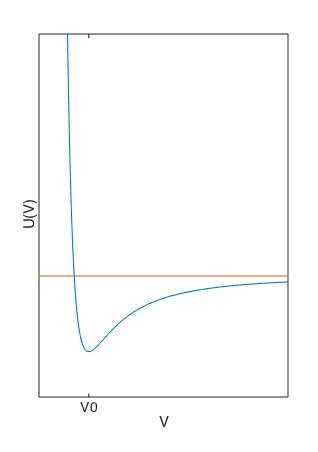
\includegraphics[width=0.2\linewidth]{Figures/UV_liquide.jpg}

\end{tabular}

\smallskip 
- Si $V<V_0$ , $P>0$ (liquide comprimé)

\smallskip
- Si $V>V_0$ , $P<0$ (liquide en dépression ; état métastable mais parfois observé !)

\medskip 


Le coefficient 
$ \chi_S = 1/V {\left.\partial V/\partial P\right|}_S \equiv  1/V \left( {\left.\partial^2 U/\partial V^2\right|}_S \right)^{-1}$ 
est très faible : les liquides sont très peu compressibles.

\medskip

Donc l'équation d'état est souvent dégénérée en  $V = V_0$.

%\qquad

%Equation d'état énergétique :

%$

\medskip

Ou en variables intensives : $\rho = \rho_0$.

\medskip



Remarque : $\rho_0$ peut dépendre de $T$, on parle alors de liquide incompressible dilatable.


\bigskip

%--------------------------------------------------------------------------------------------------
\begin{frame}{Hypothèse de l'équilibre thermodynamique local}
%--------------------------------------------------------------------------------------------------


Les lois d'état issues de la thermodynamiques sont valables dans les conditions de l'équilibre 
(repos, P T uniformes, pas de force extérieure).

\medskip


Peut-on les utiliser pour décrire l'état local d'un fluide aux propriétés non uniforme et éventuellement en mouvement ?

\medskip 

Hypothèse de l'équilibre thermodynamique local : 

\medskip

Avec l'approche du Milieu Continu on suppose les propriétés localement homogènes à l'échelle
d'un Volume Elémentaire Représentatif de dimension grande devant l'échelles microscopiques 
$\ell$ et petite devant l'échelle macroscopique $L$ .

\medskip 
Cette approche est justifiée sous la condition :

\smallskip
$\Knudsen \equiv \ell / L \ll 1 $

\smallskip

$\Knudsen$ est le Nombre de \textcolor{rouge}{\bf Knudsen} (nombre sans dimension).




%\smallskip

%\hfill [$\rightarrow$ cf. expérience de mesure de la masse volumique$^\star$]

%\medskip

%Cette échelle de longueur définit l'échelle de la \textcolor{rouge}{particule fluide},  
%sur laquelle \\ la matière est dans un état local homogène ($a\ll L$).

% de quasi-équilibre thermodynamique, 
%\\
%c'est-à-dire assez grande ($a \gg \ell$) pour contenir suffisamment d'atomes ou de molécules 
%\\
%pour que cette notion de quasi-équilibre ait un sens du point de vue de la physique statistique.

\vspace{5mm}

\end{frame}





%\vspace{10mm}

\end{frame}


%
%%--------------------------------------------------------------------------------------------------
%\begin{frame}{Motivations : des défis scientifiques actuels}
%%--------------------------------------------------------------------------------------------------
%
%\small
%
%Les fluides interviennent dans de nombreuses applications et sont au c{\oe}ur d'enjeux économiques 
%et écologiques majeurs.
%
%\medskip
%
%Ils sont aussi sources de plusieurs verrous scientifiques fondamentaux, qui les associent 
%aux plus grands défis de la physique moderne, comme en témoigne le classement effectué 
%par le CNRS à l'occasion de l'année mondiale de la physique par l'ONU en 2005 :
%
%\medskip
%
%\begin{itemize}
%\item \textcolor{vert}{Les mystères de l'eau}
%\item \textcolor{rouge}{Insaisissable turbulence}
%\item \textcolor{vert}{L'obscure nature du verre}
%\item \textcolor{rouge}{Les ambiguïtés des solides liquides}
%\item Les états étranges de la matière
%\item Les frontières incertaines du monde quantique
%\item Antimatière o{\`u} es-tu ?
%\item Energie noire, la grande inconnue
%\item Le casse-tête de l'unification des forces
%\item A la poursuite des particules élémentaires
%\end{itemize}
%
%\end{frame}



%
%%==================================================================================================
%\subsubsection{Motivations}
%%==================================================================================================
%
%%--------------------------------------------------------------------------------------------------
%\begin{frame}{Motivations : des applications multiples}
%%--------------------------------------------------------------------------------------------------
%
%\small
%
%\vspace{5mm}
%
%L'intérêt pour l'étude des écoulements des fluides est motivé par de nombreuses applications, \\ entre autres :
%
%\begin{itemize}
%\item<2->
%  Aérodynamique
%\item<3->
%  Hydrodynamique
%\item<4->
%  Bio-ingénierie et systèmes biologiques
%\item<5->
%  Production d'énergie
%\item<6->
%  Géologie
%\item<7->
%  Hydraulique et hydrologie
%\item<8->
%  Météorologie
%\item<9->
%  Planétologie, astrophysique
%\item<10->
%	Gestion des ressources en eau
%\end{itemize}
%
%\begin{overprint}
%
%  \onslide<2>   
%  \begin{center}
%    \begin{picture}(45, 40)
%    \put(0, 5){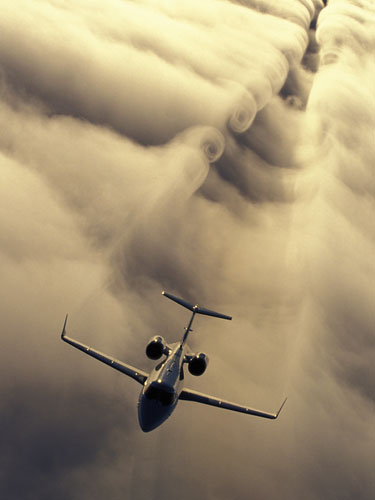
\includegraphics[width=45mm]{trailing_vortices_railtrack.jpg}}
%    \end{picture}
%  \end{center}
%
%  \onslide<3>   
%  \begin{center}
%    \begin{picture}(90, 40)
%    \put(0, 5){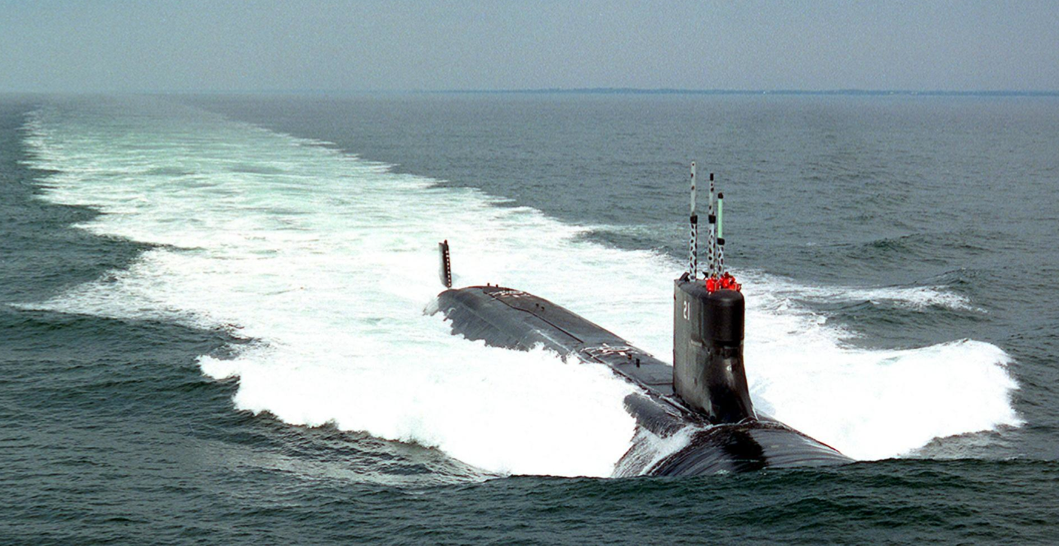
\includegraphics[width=90mm]{sous_marin.png}}
%    \end{picture}
%  \end{center}
%
%  \onslide<4>   
%  \begin{center}
%    \begin{picture}(100, 40)
%    \put(0, 5){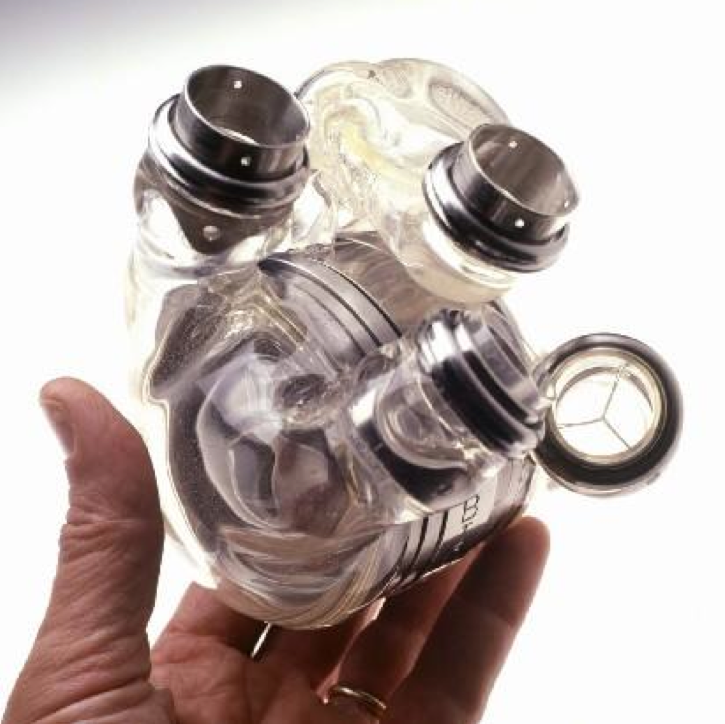
\includegraphics[width=45mm]{coeur_artificiel.png}}
%    \put(50, 5){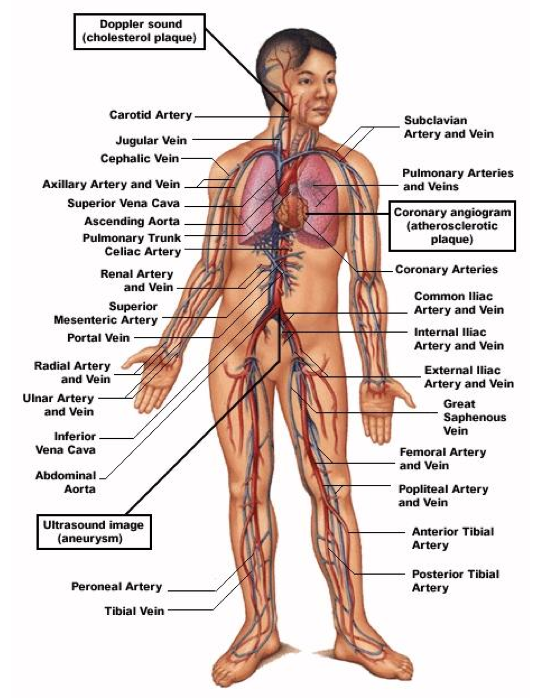
\includegraphics[width=50mm]{circulation_sang.png}}
%    \end{picture}
%  \end{center}
%
%  \onslide<5>   
%  \begin{center}
%    \begin{picture}(60, 40)
%    \put(0, 5){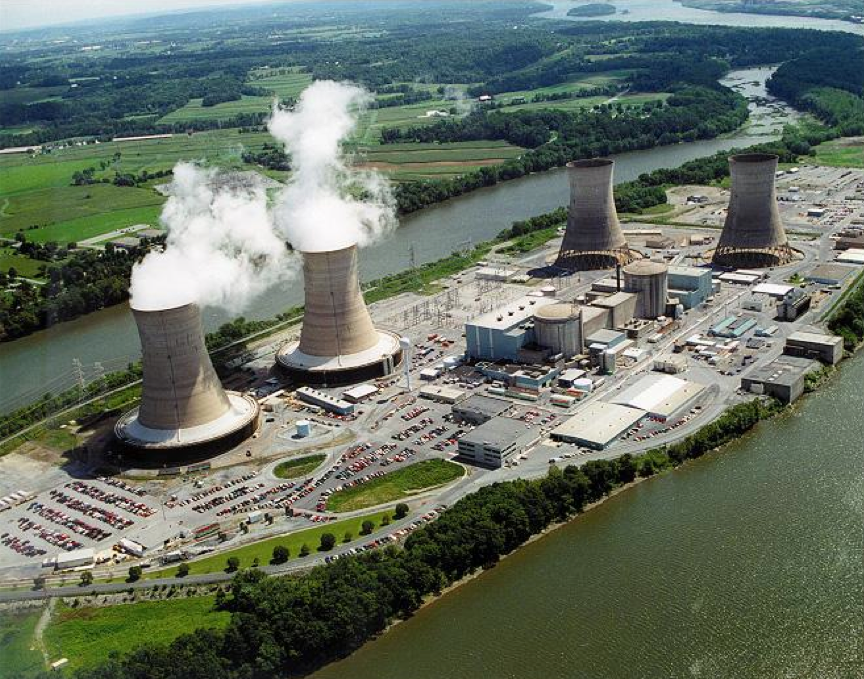
\includegraphics[width=60mm]{centrale_nucleaire.png}}
%    \end{picture}
%  \end{center}
%
%  \onslide<6>   
%  \begin{center}
%    \begin{picture}(65, 40)
%    \put(0, 5){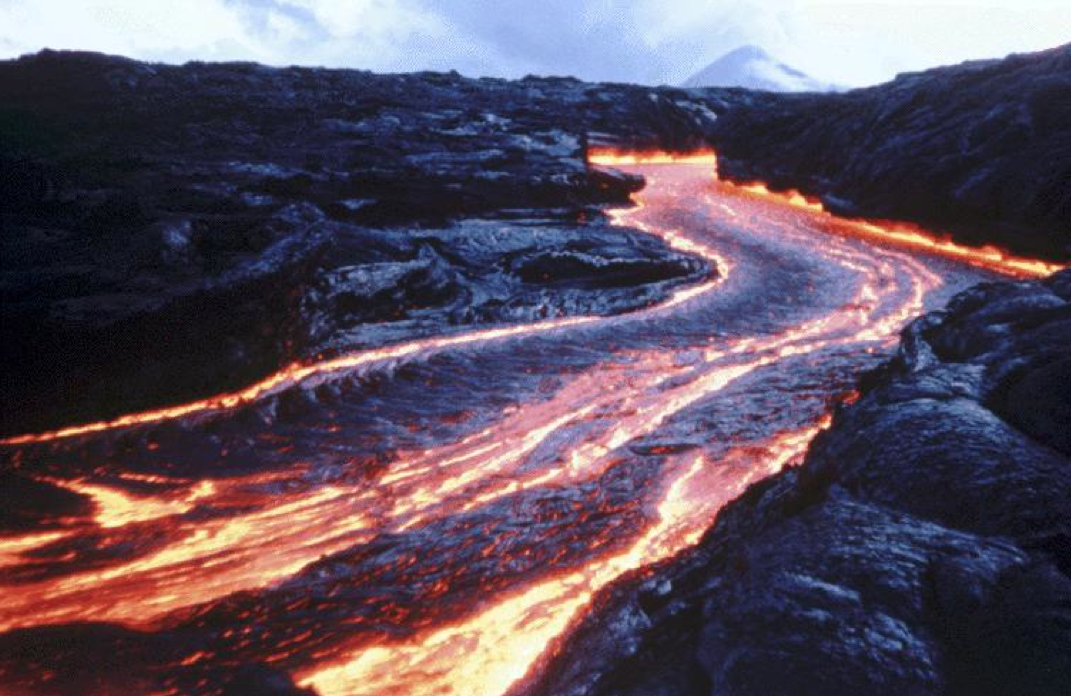
\includegraphics[width=65mm]{coulee_lave.png}}
%    \end{picture}
%  \end{center}
%
%  \onslide<7>   
%  \begin{center}
%    \begin{picture}(105, 40)
%    \put(0, 5){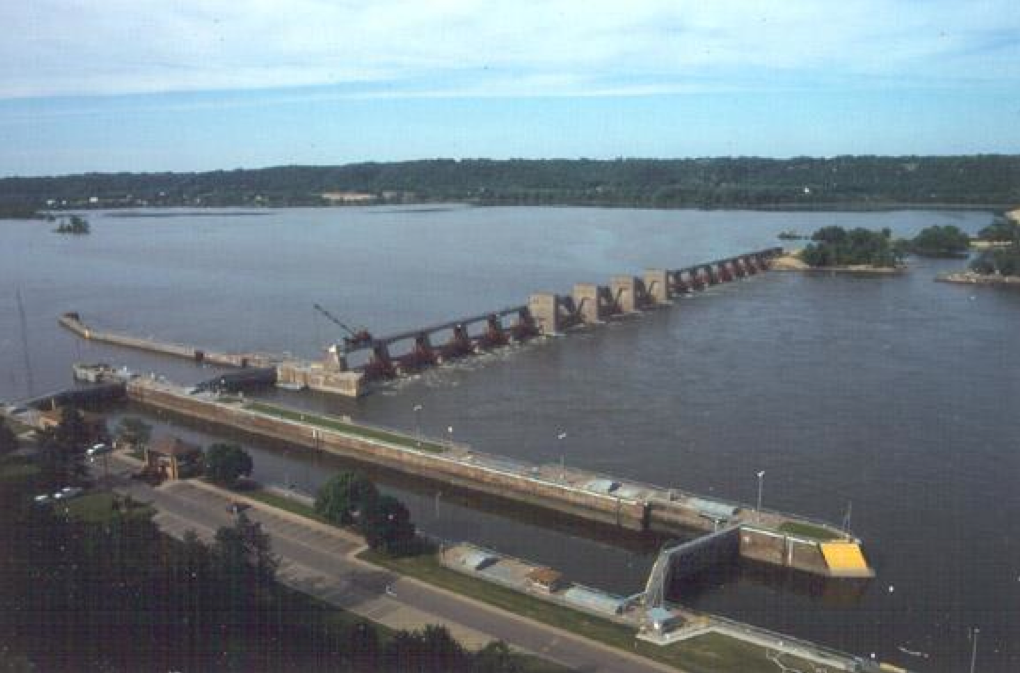
\includegraphics[height=35mm]{barrage_hydraulique.png}}
%    \put(55, 5){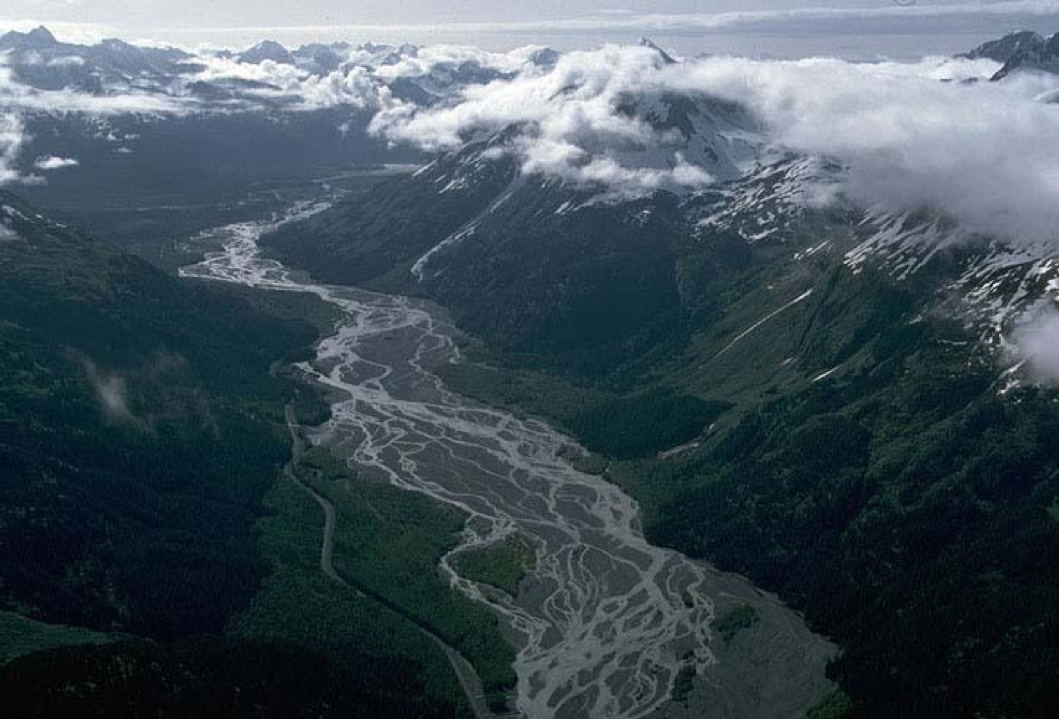
\includegraphics[height=35mm]{bassin_vallee.png}}
%    \end{picture}
%  \end{center}
%
%  \onslide<8>   
%  \begin{center}
%    \begin{picture}(100, 40)
%    \put(0, 5){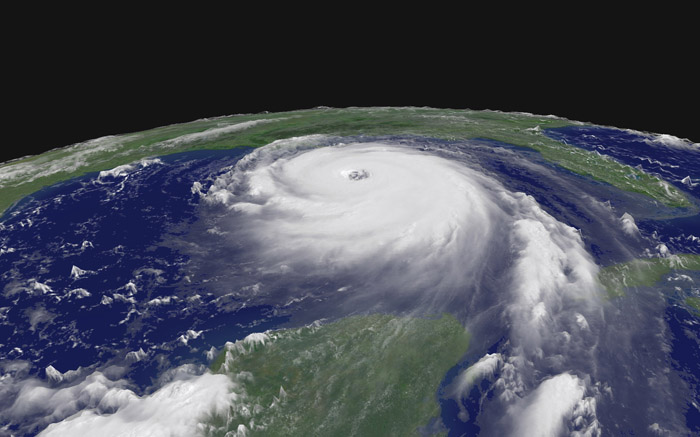
\includegraphics[height=35mm]{katrina_08-28-2005_NOAA.jpg}}
%    \put(58, 5){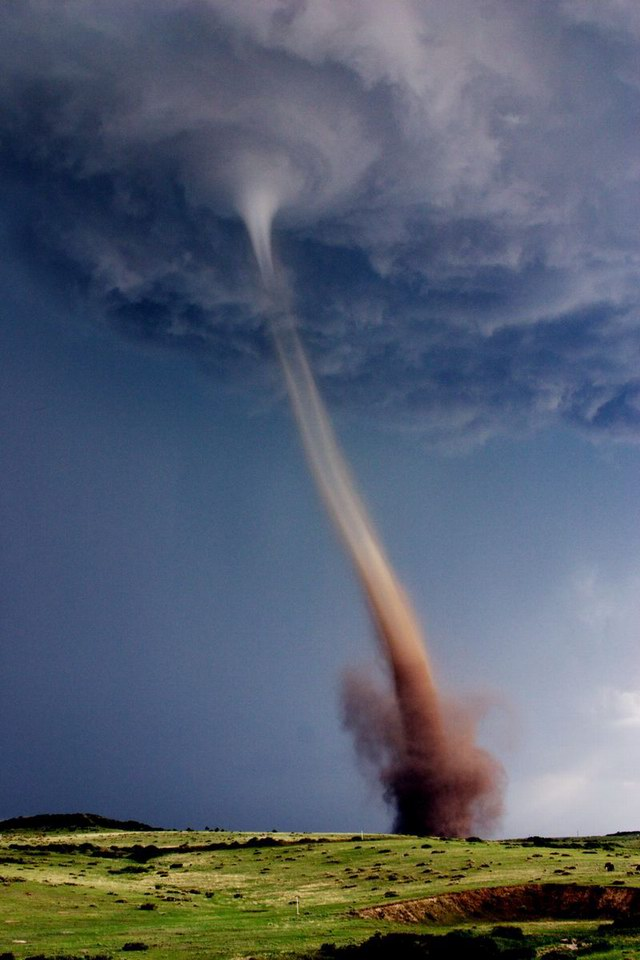
\includegraphics[height=60mm]{tornade.jpg}}
%    \end{picture}
%  \end{center}
%  
%    \onslide<9>   
%  \begin{center}
%    \begin{picture}(100, 40)
% %   \put(0, 5){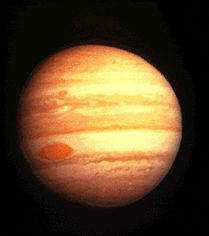
\includegraphics[height=35mm]{Jupiter.jpg}}
%  %  \put(58, 5){\includegraphics[height=60mm]{Galaxie.jpg}}
%    \end{picture}
%  \end{center}
%
%
%  \onslide<10>   
%  \begin{center}
%    \begin{picture}(100, 40)
%    \put(0, 5){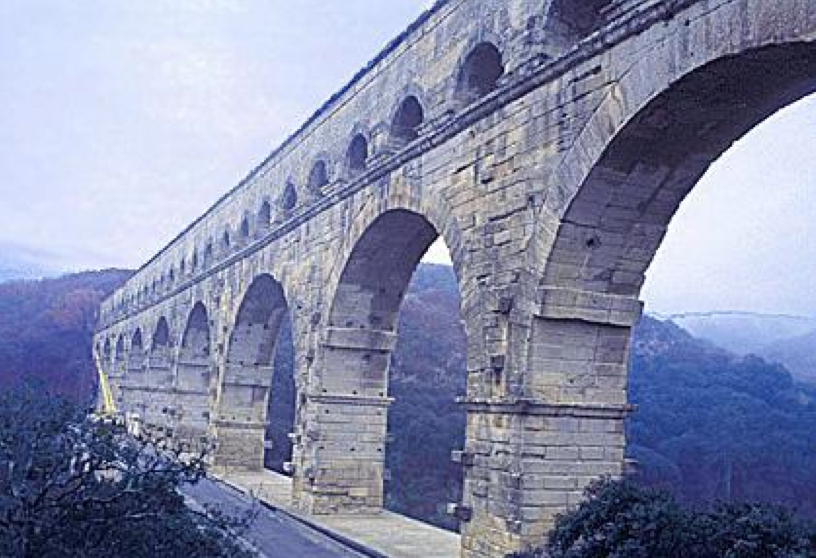
\includegraphics[height=33mm]{aqueduc.png}}
%    \put(50, 4.8){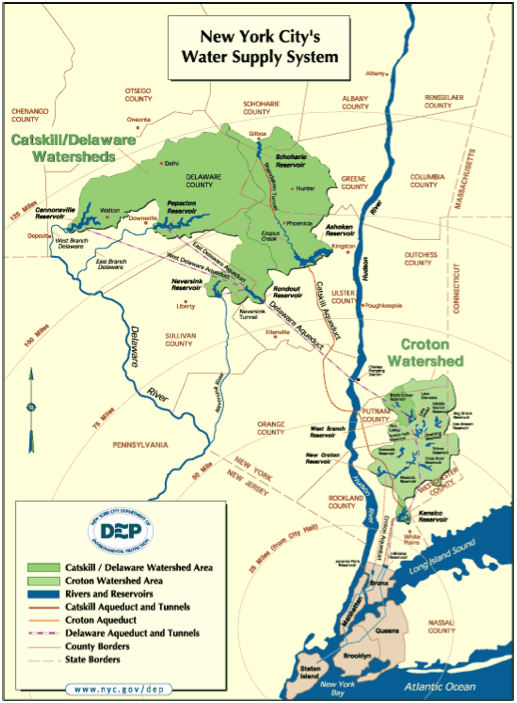
\includegraphics[height=60mm]{reseau_eau_New_York.png}}
%    \end{picture}
%  \end{center}
%
%
%\end{overprint}
%
%\end{frame}

%
%%--------------------------------------------------------------------------------------------------
%\begin{frame}{Des définitions diverses\ldots} 
%%--------------------------------------------------------------------------------------------------
%
%\small
%
%\textbf{Point de vue du physicien :} \bigskip
%
%Certains systèmes constitués d'un grand nombre d'objets solides peuvent avoir un 
%comportement fluide (et être décrits par les outils de la mécanique des fluides) :
%
%\pause
%
%\medskip
%
%\begin{itemize}[<+-| alert@+>]
%\item
%	sable (sablier)
%
%\item
%	trafic automobile, piétons	
%\item
%	galaxies, disques d'accrétion (systèmes solaires en formation)
%\item
%	boues, neige (avalanches), nuages (particules d'eau liquide ou solide)
%%\item
%%	verre ?
%%\item
%%	pâtes agroalimentaires (ketchup, dentifrice, etc.)
%\end{itemize}
%
%\end{frame}


%--------------------------------------------------------------------------------------------------
\begin{frame}{Des définitions diverses\ldots} 
%--------------------------------------------------------------------------------------------------

\small

\textbf{Point de vue du mécanicien :} \bigskip

Mécanique = science qui s'intéresse au lien entre forces et mouvements.

"Un fluide est un matériau qui, sous l'effet d'une contrainte imposée, se déforme continument".

Mais le comportement solide ou fluide peut dépendre :

\medskip

\pause


\textbf{De la valeur de la contrainte exercée :}

\begin{itemize}[<+-| alert@+>]

\item Dentifrice, ketchup,...

\item Neige (avalaches)

\item mousses,...

\end{itemize}

\medskip 

\pause

\textbf{De la durée d'observation :}

\begin{itemize}[<+-| alert@+>]
\item 
	Glacier (glace : eau solide) : 
	vitesse de coulée, %si épaisseur supérieure à 50 m, 
	environ 10 cm à 10 m / jour

\item
	Bitume (goudron) :
	Expérience de l'université de Brisbane, 9 gouttes depuis 1927.
	
\item Verre ?

\item 

	\hyperlink{frame:manteau_terrestre}{manteau terrestre$^\star$}
	(roches solides) : comportement fluide à l'échelle de temps géologique 
	\\ ($\sim$ million d'années) avec des déformations de l'ordre du cm / an 
	(tectonique des plaques de surface), en particulier 
	sous l'effet du phénomène de convection thermique dans le manteau.
% qui se comporte donc comme un fluide compressible (dilatable) !

\item Solution de Maïzena 

Une expérience amusante : 
\href{https://www.youtube.com/watch?v=f2XQ97XHjVw}{
\color{blue}{https://www.youtube.com/watch?v=f2XQ97XHjVw}
}


\end{itemize}

%\textbf{De la durée caractéristique de la contrainte :}


\medskip
\pause


L'étude de la relation entre contraintes et déformation s'appelle la rhéologie.

\end{frame}


}



